\documentclass[10pt]{beamer}

\usetheme{metropolis}
\usepackage{appendixnumberbeamer}

\usepackage{booktabs}
\usepackage{multirow}
\usepackage[scale=2]{ccicons}

\usepackage{pgfplots}
\usepgfplotslibrary{dateplot}

\usepackage{xspace}
\newcommand{\themename}{\textbf{\textsc{metropolis}}\xspace}
\usepackage{tabularx}

\usepackage[utf8]{inputenc}
\usepackage[brazilian]{babel}

\usepackage{blindtext}
\usepackage[portuguese, noend, plain, linesnumbered]{algorithm2e}

\setbeamercolor{background canvas}{bg=white}

\title{}
\subtitle{Uso de Redes de Função de Base Radial e Cadeias de Markov para detecção online de mudanças de conceito em fluxos contínuos de dados}
\date{}
\author{\textbf{Discente:} Ruivaldo Neto \newline \textbf{Orientador:} Ricardo Rios}
\institute{Universidade Federal da Bahia \newline Departamento de Ciência da Computação \newline Programa de Pós-Graduação em Ciência da Computação \newline\newline Contato: rneto@rneto.dev \newline\newline 16 de Dezembro de 2019}

\titlegraphic{%
  \begin{picture}(0,0)
    \put(330, 28){\makebox(0,0)[rt]{
\includegraphics[scale=0.25]{logo.png}}}
  \end{picture}
}

\begin{document}

\maketitle

\begin{frame}{Roteiro}
  \setbeamertemplate{section in toc}[sections numbered]
  \begin{minipage}{\textwidth}
    \tableofcontents
  \end{minipage}
\end{frame}

\section{Introdução}

\begin{frame}{Introdução}
    \begin{itemize}
        \item<1 -> Avanços tecnológicos recentes contribuiram para um aumento exponencial no volume de dados produzidos por sistemas computacionais \cite{idc_report}.
        \item<1 -> Parte significativa desses dados é produzida atráves de \alert{Fluxos Contínuos de Dados (FCDs)}: sequências \alert{ininterruptas} e \alert{potencialmente infinitas} de eventos \cite{Aggarwal:2006:DSM:1196418}.
        \item<1 -> FCDs estão presentes em diversos domínios de aplicação:
        \begin{itemize}
            \item Análise do Mercado Financeiro;
            \item Gestão de redes de telecomunicação;
            \item Detecção de intrusos;
            \item Monitoramento de tráfico, etc.
        \end{itemize}
      \end{itemize}
\end{frame}

\begin{frame}{Introdução}
    \begin{itemize}
        \item<1 -> Técnicas de \alert{Aprendizado de Máquina (AM)} têm sido aplicadas para extrair informações úteis desses grandes conjuntos de dados.
        \item<1 -> Cenários com FCDs limitam a aplicação de técnicas de AM, pois impõem restrições de tempo de resposta, de uso dos recursos computacionais e apresentam comportamento \alert{não estacionário}.
        \item<1 -> Em cenários \alert{não estacionários}, o contexto do processo gerador e/ou a distribuição dos dados podem sofrer alterações (\alert{mudanças de conceito}) ao longo do tempo.
        \item<1 -> A ocorrência de \alert{mudanças de conceito} (\textit{concept drifts}) pode impactar negativamente a acurácia das técnicas aplicadas.
      \end{itemize}
\end{frame}

\begin{frame}{Introdução}
    \begin{itemize}
        \item<1 -> A atualização periódica de modelos, apesar de computacionalmente ineficiente, foi utilizada inicialmente como estratégia para mitigar a perda de acurácia causada por mudanças de conceito.
        \item<1 -> A fim de obter maior eficiência e precisão, pesquisadores propuseram novos métodos de detecção de mudança de conceito baseados em monitoramento.
      \end{itemize}
\end{frame}


\begin{frame}{Introdução}
    \begin{itemize}
        \item<1 -> Entretanto, esses métodos ainda apresentam limitações ao serem aplicados em cenários com FCDs \cite{Aggarwal:2006:DSM:1196418}:
        \begin{itemize}
            \item<1 -> Necessidade de rotulação;
            \item<1 -> Eficiência computacional (tempo de resposta e uso de recursos).
        \end{itemize}
      \end{itemize}
\end{frame}

\begin{frame}{Introdução}
    \begin{itemize}
        \item<1 -> Visando superar essas limitações, este trabalho propõe um novo método de detecção de mudanças de conceito baseado em \alert{Redes de Função de Base Radial (redes RBF) e Cadeias de Markov}, denominado \textbf{\alert{RBFChain}}.
        \item<1 -> O método proposto se diferencia por detectar mudanças em \alert{tempo de execução}, de forma computacionalmente \alert{eficiente} e \alert{independente de rótulos}.
    \end{itemize}
\end{frame}

\section{Fundamentação Teórica}

\begin{frame}{Fluxos Contínuos de Dados e Aprendizado de Máquina}
    \begin{itemize}
        \item<1 -> \alert{Fluxos Contínuos de Dados (FCDs)} são sequências ininterruptas e potencialmente infinitas de eventos \cite{Aggarwal:2006:DSM:1196418}.
        \item<1 -> Não podem ser armazenados em sua totalidade e, por serem de alta frequência, devem ser analisados em tempo real.
        \item<1 -> Algoritmos supervisionados \cite{Domingos:2000:MHD:347090.347107, Bifet:2013:EDS:2480362.2480516, Wang:2003:MCD:956750.956778, Aggarwal:2004:DCD:1014052.1014110, Gama:2003:ADT:956750.956813} e não-supervisionados \cite{Aggarwal:2003:FCE:1315451.1315460, Ackermann:2012:SCA:2133803.2184450, Kranen:2011:CIM:2134350.2134352} da área de AM foram adaptados para atenderem a essas restrições.
        \item<1 -> Contudo, essas especializações não tratam a ocorrência de \alert{mudanças de conceito}.
      \end{itemize}
\end{frame}

\begin{frame}{Mudança de Conceito}
    \begin{itemize}
        \item<1 -> A Teoria Bayesiana de Decisão \cite{Duda:2000:PC:954544} é comumente utilizada para descrever a tarefa de classificação e pode ser utilizada para formalizar a noção de \alert{mudança de conceito}.
        \item<1 -> Considerando que $p_{t_0}$ e $p_{t_1}$ denotam as distribuições de probabilidades conjuntas nos instantes $t_0$ e $t_1$, é possível afirmar que há mudança de conceito entre os instantes $t_0$ e $t_1$ se:
        \begin{equation} \label{eq:3}
            {\exists}X : p_{t_0}(X, c) \ne p_{t_1}(X, c)
        \end{equation}
        \item<1 -> Ou seja: um conjunto de dados possui resultados esperados legítimos em $t_0$, mas este mesmo conjunto passa a ter resultados esperados diferentes, também legítimos, em $t_1$ \cite{Kolter:2007:DWM:1314498.1390333}.
    \end{itemize}
\end{frame}

\begin{frame}{Mudança de Conceito}
    \begin{itemize}
        \item<1 -> As mudanças de conceito podem ser categorizadas como \alert{Virtuais} ou \alert{Reais} \cite{Gama:2014:SCD:2597757.2523813}:
        \begin{itemize}
        \item<1 -> \alert{Mudanças Virtuais} são causadas por alterações na probabilidade a priori das classes, $P(c)$, e não alteram os conceitos-alvo.
        \item<1 -> \alert{Mudanças Reais} surgem a partir de alterações na probabilidade a posteriori, $p(c|X)$, e modificam os resultados esperados.
        \end{itemize}
    \end{itemize}
\end{frame}

\begin{frame}{Mudança de Conceito}
\begin{figure}[H]
    \begin{center}
        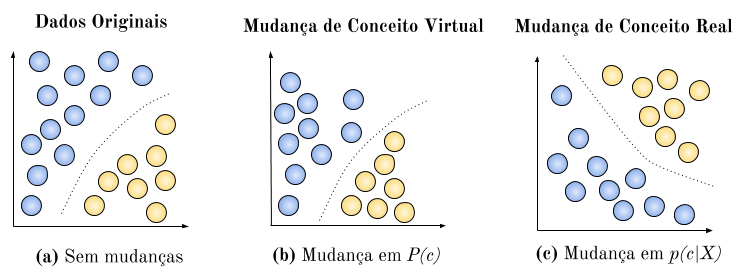
\includegraphics[scale=0.5]{imagens/concept_drift.png}
        \caption{Mudança de Conceito Virtual vs. Mudança de Conceito Real}
        \label{fig:real_and_virtual_concept_drift}
    \end{center}
\end{figure}
\end{frame}

\begin{frame}{Mudança de Conceito}
    \begin{itemize}
        \item<1 -> As mudanças de conceito podem ocorrer de forma \alert{abrupta}, \alert{gradual}, \alert{incremental} ou \alert{recorrente} \cite{Zliobaite:2010}.
    \end{itemize}
    \begin{figure}[H]
        \begin{center}
            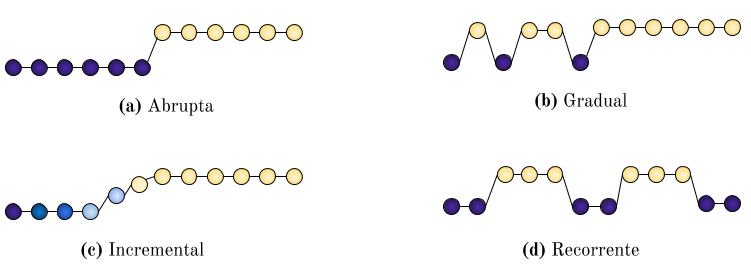
\includegraphics[scale=0.5]{imagens/concept_drift_patterns.png}
            \caption{Padrões de ocorrência de Mudanças de Conceito}
            \label{fig:concept_drift_patterns}
        \end{center}
    \end{figure}
\end{frame}

\begin{frame}{Algoritmos para Detecção de Mudança de Conceito}
    \begin{itemize}
        \item<1 -> Os algoritmos para Detecção de Mudanças de Conceito se dividem em duas categorias, conforme a necessidade de rotulação dos dados \cite{Zliobaite:2010}:
        \begin{itemize}
        \item<1 -> \alert{Explícitos/Supervisionados}: \textbf{Dependem} da rotulação dos dados. Realizam a detecção a partir do monitoramento de medidas de performance como taxa de erro e acurácia.
        \item<1 -> \alert{Implícitos/Não Supervisionados}: \textbf{Independem} da rotulação dos dados. Realizam a detecção através do monitoramento de características dos próprios dados ou de indicadores produzidos pelas técnicas de aprendizado aplicadas.
        \end{itemize}
    \end{itemize}
\end{frame}

\begin{frame}{Ferramenta: MOA}
    \begin{itemize}
        \item<1 -> Principal framework para mineração de dados em fluxos contínuos.
        \item<1 -> Permite implementar e validar novos métodos de detecção de mudança de conceito de forma trivial.
    \end{itemize}
    \begin{figure}[H]
        \begin{center}
            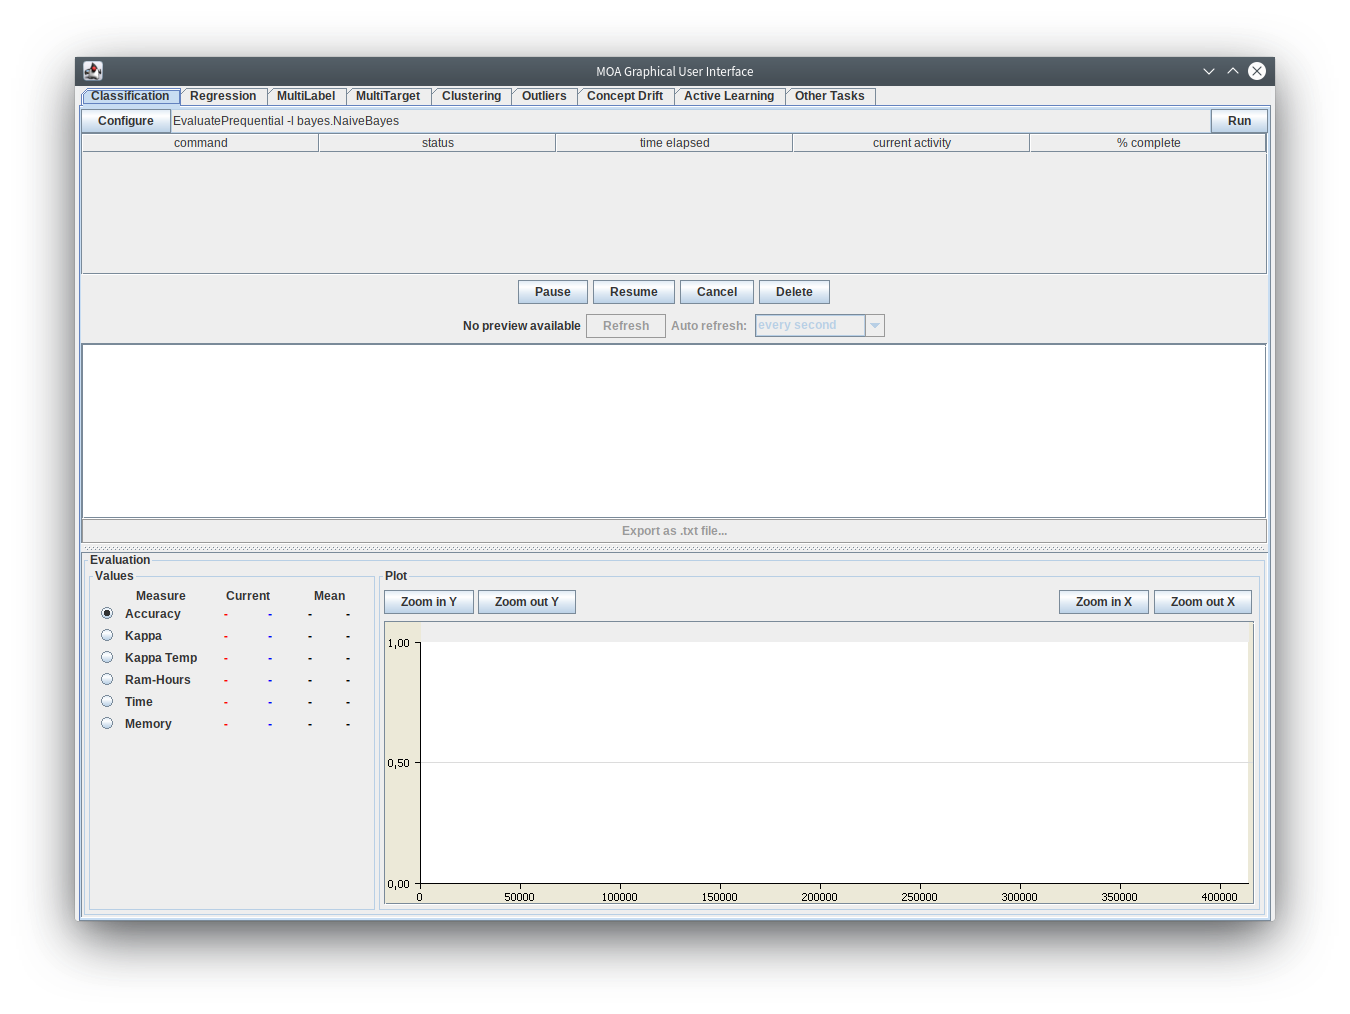
\includegraphics[scale=0.25]{imagens/moa.png}
        \end{center}
    \end{figure}
\end{frame}

\begin{frame}{Mudança de Conceito - RBFChain}
    \begin{itemize}
        \item<1 -> O método proposto neste trabalho é capaz de identificar mudanças \alert{sob qualquer padrão de ocorrência}.
        \item<1 -> Por ser independente de rótulos, considera todas mudanças identificadas como \alert{mudanças reais}.
        \item<1 -> Implementado e validado através da plataforma MOA.
    \end{itemize}
\end{frame}

\begin{frame}{Redes de Função de Base Radial}
    \begin{itemize}
        \item<1 -> \alert{Redes de Função de Base Radial} são redes neurais cujo principal diferencial é a forma de ativação: pois é realizada através do cálculo da distância entre o evento e um centro definido \cite{Braga:RedesNeuraisTeoriaAplicacoes}.
        \item<1 -> A arquitetura de uma rede RBF, em sua forma mais básica, envolve três camadas:
        \begin{itemize}
            \item<1 -> \alert{Entrada}: Recepciona os dados e encaminha para camada intermediária.
            \item<1 -> \alert{Intermediária}: Composta por funções de ativação de base radial que atuam como neurônios.
            \item<1 -> \alert{Saída}: Pondera os resultados da camada intermediária, agregando-os linearmente para compor a resposta final da rede.
        \end{itemize}
        \item<1 -> Na literatura, as funções Gaussianas são as funções de ativação mais usuais em redes RBF.
      \end{itemize}
\end{frame}

\begin{frame}{Redes de Função de Base Radial}
    \begin{figure}[H]
    \begin{center}
        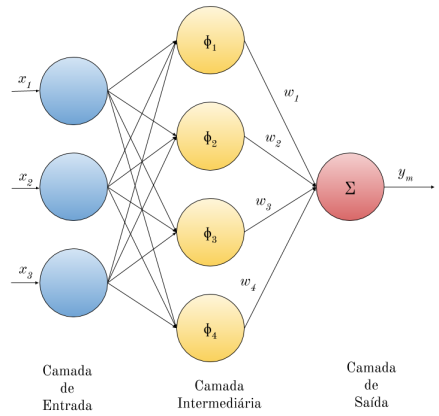
\includegraphics[scale=0.65]{imagens/rbf_arq.png}
    \end{center}
    \end{figure}
\end{frame}

\begin{frame}{Redes de Função de Base Radial}
    \begin{itemize}
        \item<1 -> O RBFChain utiliza uma rede RBF adaptada, composta apenas pelas camadas inicial e intermediária.
        \item<2 -> O processo de ativação realizado na camada intermediária produz, implicitamente, grupos a partir das observações recebidas ao longo do tempo.
        \item<3 -> Mudanças de conceito são identificadas quando o grupo ativo deste agrupamento é alterado.
      \end{itemize}
\end{frame}


\begin{frame}{Cadeias de Markov}
    \begin{itemize}
        \item<1 -> Equações determinísticas não podem ser utilizadas para descrever sistemas com múltiplos caminhos evolutivos;
        \item<1 -> Nestes casos, \alert{processos estocásticos} são utilizados \cite{taylor1998introduction};
        \item<1 -> Um \alert{processo estocástico} é uma coleção de variáveis aleatórias indexadas no tempo: $\left\{ X _ { t } : t \in T \right\}$;
        \item<1 -> Considerando que o processo estocástico esteja no estado $s_i$ e no tempo $t - 1$, a probabilidade
        do processo estar no estado $s_j$ no tempo $t$ é dada pela Equação \ref{eq:prob_proc_estoc}:
        \begin{equation}
            \label{eq:prob_proc_estoc}
            \mathbb { P } \left( X _ { t } = s _ { j } | X _ { t - 1 } = s _ { i } , \ldots , X _ { 0 } = s _ { 0 } \right)
        \end{equation}
      \end{itemize}
\end{frame}

\begin{frame}{Cadeias de Markov}
    \begin{itemize}
        \item<1 -> Uma \alert{Cadeia de Markov}, ou \alert{Processo de Markov}, é um processo estocástico no qual a probabilidade do estado em um dado período de tempo depende apenas do estado no período imediatamente anterior:
        \begin{equation}
            \label{eq:markov}
            \mathbb { P } \left( X _ { t } = s _ { j } | X _ { t - 1 } = s _ { i } , \ldots , X _ { 0 } = s _ { 0 } \right) = \mathbb { P } \left( X _ { t } = s _ { j } | X _ { t - 1 } = s _ { i } \right) = p _ { i j }
        \end{equation}
      \end{itemize}
\end{frame}

\begin{frame}{Cadeias de Markov}
    \begin{itemize}
        \item<1 -> Um processo de Markov pode assumir os estados $a_1, a_2, \ldots, a_r$, de tal modo que a probabilidade de transição de um estado $a_i$ para um estado $a_j$ seja $P_{ij}$ (um valor dependente apenas de $i$ e $j$);
        \item<1 -> Portanto, é viável elaborar uma matriz com as probabilidades de todas transições (matriz estocástica) - Equação \ref{eq:matriz_estocastica}:
        \begin{equation}
            \label{eq:matriz_estocastica}
            P = \left[ \begin{array} { c c c c } { P _ { 11 } } & { P _ { 12 } } & { \dots } & { P _ { 1 r } } \\ { P _ { 21 } } & { P _ { 22 } } & { \dots } & { P _ { 2 r } } \\ { \vdots } & { \vdots } & { \vdots } & { \vdots } \\ { P _ { r 1 } } & { P _ { r 2 } } & { \cdots } & { P _ { r r } } \end{array} \right]
        \end{equation}
      \end{itemize}
\end{frame}

\begin{frame}{Cadeias de Markov}
    \begin{itemize}
        \item<1 -> O RBFChain utiliza uma Cadeia de Markov para modelar o agrupamento criado na rede RBF.
        \item<2 -> Os grupos formados representam os estados do modelo markoviano e as mudanças (ativações) entre estes grupos, as transições.
        \item<3 -> Estas mudanças são refletidas no modelo através do aumento da probabilidade  correspondente e a diminuição proporcional das outras transições. Estas alterações são realizadas respeitando a condição $0 \leq P_{ij} \leq 1$.
      \end{itemize}
\end{frame}

\begin{frame}{Trabalhos Relacionados}
    \begin{itemize}
        \item<1 -> Pesquisa na literatura em busca de trabalhos que propõem métodos para identificação de mudanças de conceito em fluxos contínuos de dados, de forma online e independente de rótulos.
        \item<1 -> Também foram estudadas técnicas que pudessem subsidiar o desenvolvimento de novos algoritmos que atendam a esses requisitos.
    \end{itemize}
\end{frame}

\begin{frame}{Trabalhos Relacionados}
    \begin{itemize}
        \item<1 -> Análise dos algoritmos \alert{Implícitos/Não Supervisionados} da subcategoria \alert{Detecção de Novidade / Métodos de Agrupamento}.
        \item<1 -> Análise dos métodos para detecção de \textit{Change Points} em séries temporais que atuam de forma online:
        \begin{itemize}
            \item<1 -> Modelos autoregressivos;
            \item<1 -> Séries com autosimilaridade e periodicidade.
        \end{itemize}
        \item<1 -> Análise da aplicação de algoritmos de agrupamento estáveis.
        \item<1 -> Identificação de lacuna de pesquisa.
      \end{itemize}
\end{frame}

\section{RBFChain}

\begin{frame}{Visão Geral}
    \begin{itemize}
        \item<1 -> O RBFChain atua diretamente sobre o fluxo de dados e é composto por dois componentes principais: uma Rede de Função de Base Radial (RBF) adaptada e uma Cadeia de Markov.
      \end{itemize}
\end{frame}

\begin{frame}{Visão Geral}
        \begin{figure}[H]
            \begin{center}
                
\includegraphics[scale=0.45]{imagens/arquitetura_rbfchain.png}
            \end{center}
        \end{figure}
\end{frame}


\begin{frame}{Execução de exemplo}
    \begin{itemize}
        \item $S = {0.11, 0.12, 0.13, 0.33, 0.34, 0.45, 0.6, 0.33, 0.25, 0.14, 0.11, 0.15}$
        \item $\sigma = 3, \lambda = 0.8, \alpha = 0.25, \delta = 0.5$
    \end{itemize}
    \begin{figure}[H]
        \begin{center}
            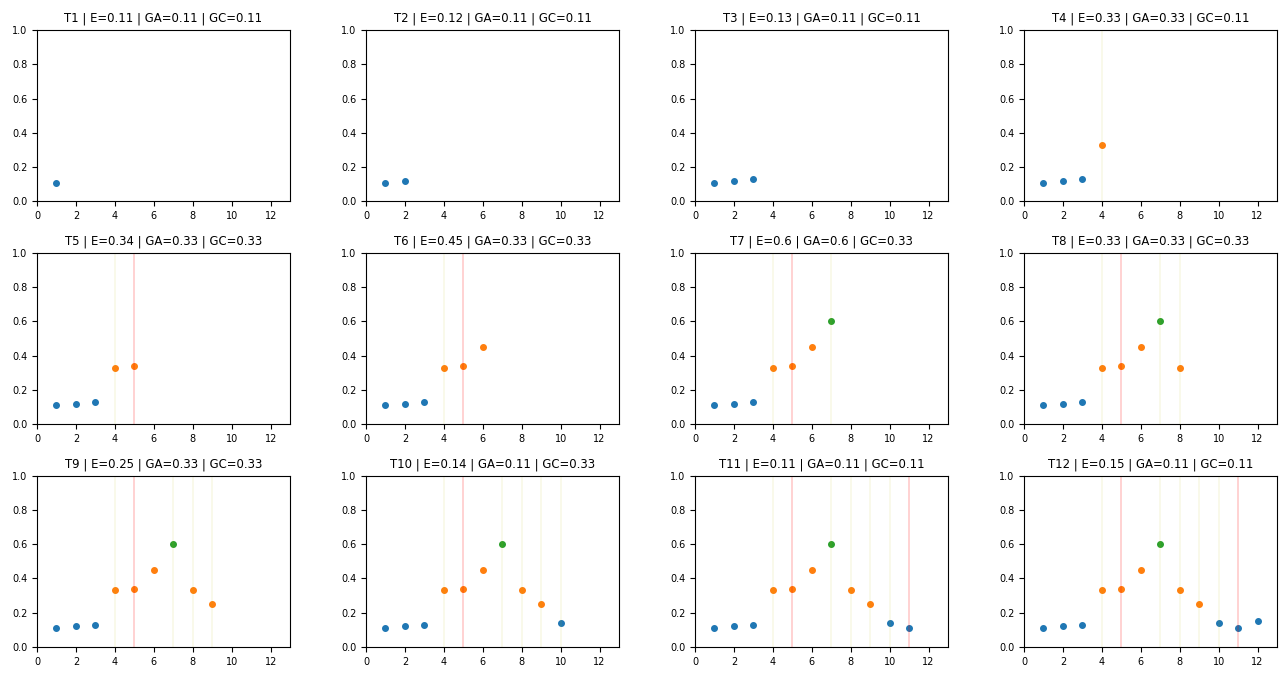
\includegraphics[width=\textwidth]{imagens/funcionamento_algoritmo.png}
        \end{center}
    \end{figure}
\end{frame}

\begin{frame}{Execução de exemplo}
    \begin{figure}[H]
        \begin{center}
            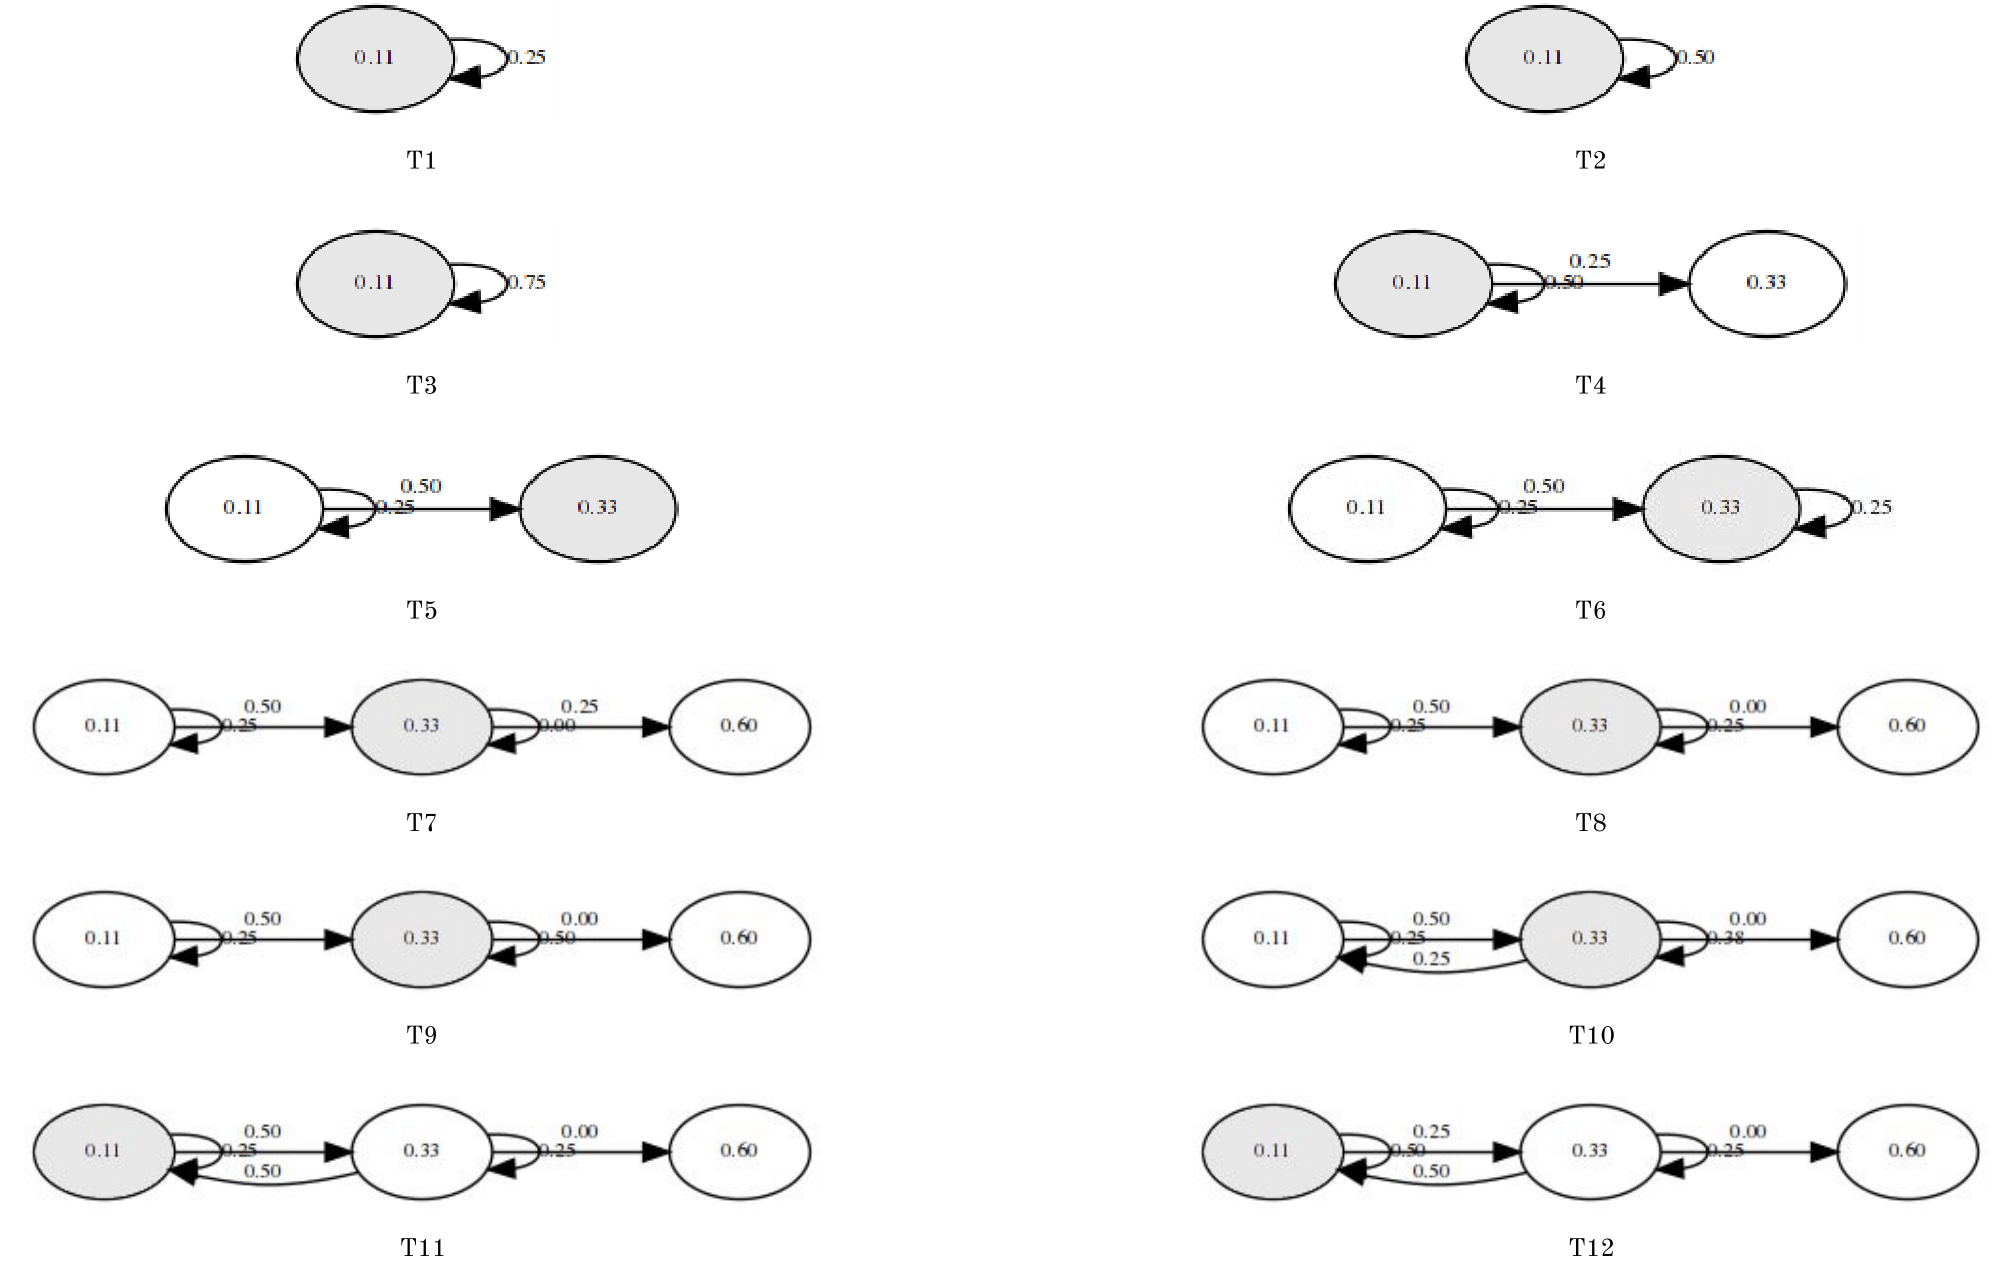
\includegraphics[width=\textwidth]{imagens/evolucao_markov.png}
        \end{center}
    \end{figure}
\end{frame}


\section{Experimentos}

\begin{frame}{Dados Sintéticos}
    \begin{figure}[ht]
        \begin{center}
            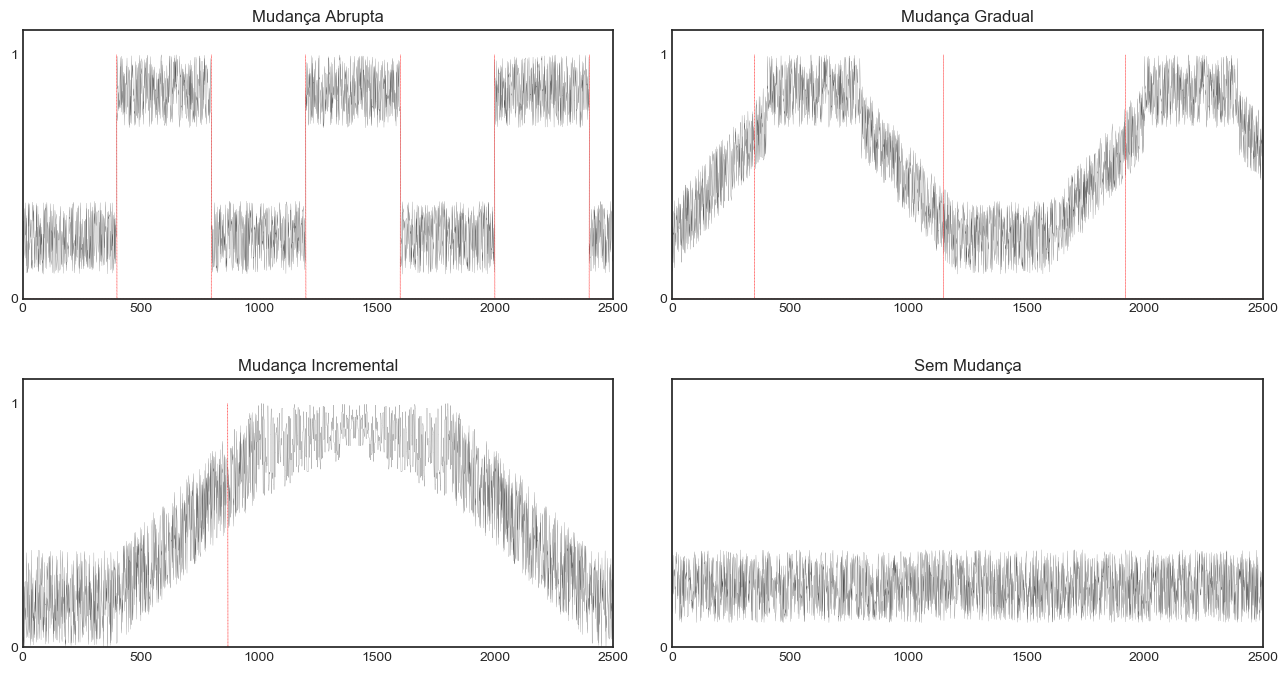
\includegraphics[width=\textwidth]{imagens/conjuntos_dados_sinteticos.png}
        \end{center}
    \end{figure}
\end{frame}


\begin{frame}{Dados Sintéticos - Critérios de Avaliação}
    \begin{table}[h]
        \centering
        \begin{tabularx}{\textwidth}{ll}
        \toprule
        Indicador & Observação \\
        \midrule
        TP       &  \textbf{Tempo de Processamento} por instância (média em seg.). \\
        MR       &  \textbf{Mudanças Reais} existentes no conjunto de dados. \\
        VP       &  \textbf{Verdadeiro Positivo}. Quantidade de detecções corretas. \\
        FP       &  \textbf{Falso Positivo}. Quantidade de detecções errôneas. \\
        ATR      &  \textbf{Atraso de detecção}. \\
                 &  Quantidade média de instâncias até a detecção. \\
        \bottomrule
        \end{tabularx}
    \end{table}
\end{frame}

\begin{frame}{Dados Sintéticos - Resultado: Sem mudanças de conceito}
    \begin{table}[h]
        \centering
        \begin{tabular}{llllll}

        \toprule
        Algoritmo              & TP                     & MR                     & VP                     & FP                     & ATR                    \\
        \midrule
        RBFChain               & 0.013                  & 0                      & 0                      & 0                      & ---                    \\
        ADWIN                  & 0.025                  & 0                      & 0                      & 0                      & ---                    \\
        CUSUM                  & 0.016                  & 0                      & 0                      & 0                      & ---                    \\
        DDM                    & 0.014                  & 0                      & 0                      & 0                      & ---                    \\
        EDDM                   & 0.013                  & 0                      & 0                      & 0                      & ---                    \\
        EWMA                   & 0.014                  & 0                      & 0                      & 0                      & ---                    \\
        HDDMA                  & 0.017                  & 0                      & 0                      & 0                      & ---                    \\
        PageHinkley            & 0.015                  & 0                      & 0                      & 0                      & ---                    \\
        SeqDrift1              & 0.017                  & 0                      & 0                      & 0                      & ---                    \\
        \bottomrule

        \end{tabular}
    \end{table}
\end{frame}

\begin{frame}{Dados Sintéticos - Resultado: Sem mudanças de conceito}
    \begin{itemize}
        \item Todos algoritmos testados demonstraram tolerância a ruídos e não indicaram nenhum falso positivo.
        \item RBFChain obteve a melhor média em tempo de processamento, juntamente com o EDDM.
    \end{itemize}
\end{frame}

\begin{frame}{Dados Sintéticos - Resultado: Sem mudanças de conceito}
    \begin{figure}[t]
        \begin{center}
            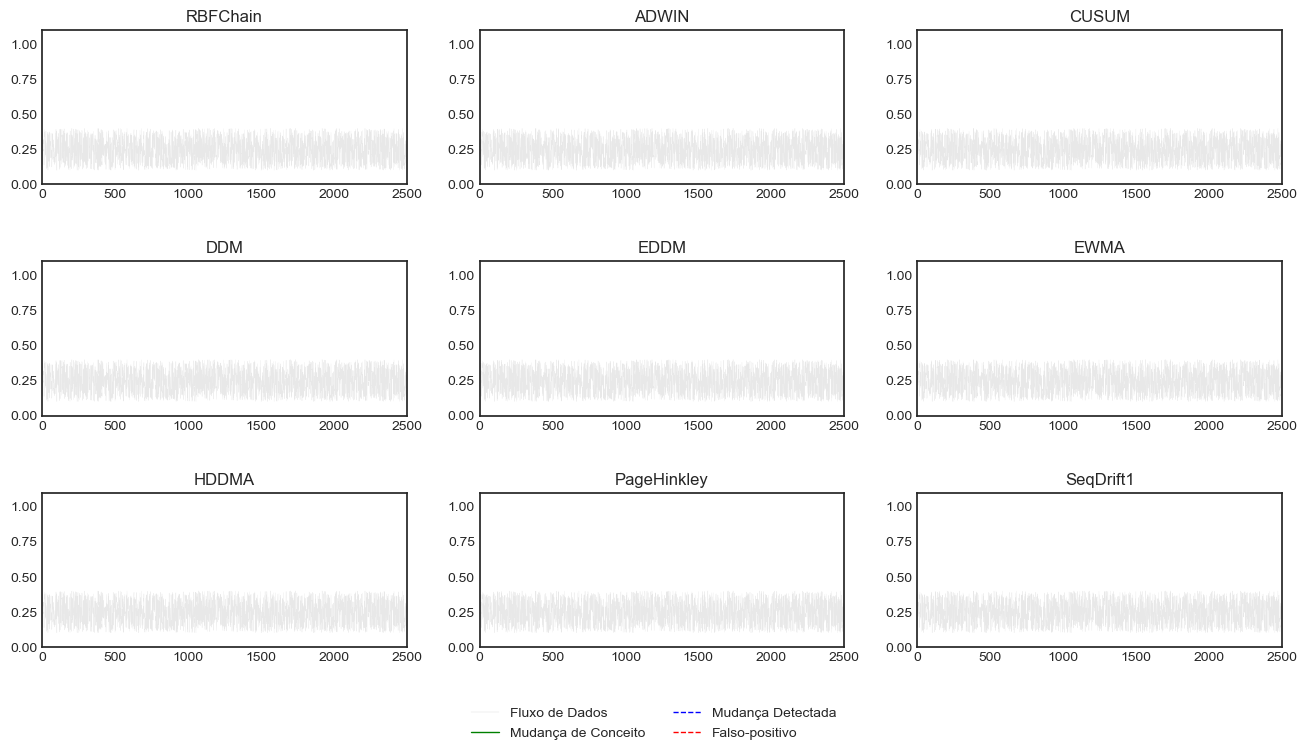
\includegraphics[width=\textwidth]{imagens/nochange.png}
        \end{center}
    \end{figure}
\end{frame}

\section{Conclusões e Trabalhos Futuros}

\begin{frame}{Lorem Ipsum}
    \begin{itemize}
        \item<1 -> A:
        \begin{itemize}
            \item<2 -> A1;
            \item<2 -> A2.
        \end{itemize}
        \item<3 -> B
      \end{itemize}
\end{frame}

\begin{frame}[allowframebreaks]{Referências}

  \bibliography{slides}
  \bibliographystyle{abbrv}

\end{frame}

\end{document}
